\documentclass{beamer}

\mode<presentation>
{
  \usetheme{CambridgeUS}
  \setbeamercovered{transparent}
}

\usepackage{amsmath}
\usepackage{verbatim}
\usepackage{color}


% The text in square brackets is the short version of your title and will be used in the
% header/footer depending on your theme.
\title[Generalized Reed-Solomon Codes]{Generalized Reed-Solomon Codes}

% Sub-titles are optional - uncomment and edit the next line if you want one.
% \subtitle{Why does sub-tree crossover work?}

% The text in square brackets is the short version of your name(s) and will be used in the
% header/footer depending on your theme.
\author[McCall]{John McCall}
\institute[U of Minn, Morris]
{
  Division of Science and Mathematics \\
  University of Minnesota, Morris \\
  Morris, Minnesota, USA
}

\AtBeginSection[]
{
  \begin{frame}<beamer>
    \frametitle{Outline}
    \tableofcontents[currentsection, hideothersubsections]
  \end{frame}
}

\begin{document}


\definecolor{greyCode}{gray}{.75}

\newcommand{\f}[1]{
	\colorbox{greyCode}{\texttt{#1}}
}


\begin{frame}
	\titlepage
\end{frame}

\section*{Overview}

\begin{frame}
	\frametitle{Overview}
	\begin{itemize}
		\item Data transmission has become vital in today's society.
		
		\item Transmission methods are not perfect.
		
		\item Error correcting codes help to alleviate the burden of transmission.
	\end{itemize}
	
\end{frame}

\begin{frame}
	\frametitle{Outline}
	\tableofcontents[hideallsubsections]
\end{frame}

\section{Defining the Playing Field}

\begin{frame}
	\frametitle{Introducing $\mathbb{F}_{64}$}
	The 64 symbols chosen to be our elements.
    % Taken From: http://www.asciitable.com/
	
	\begin{figure}
	\centering
	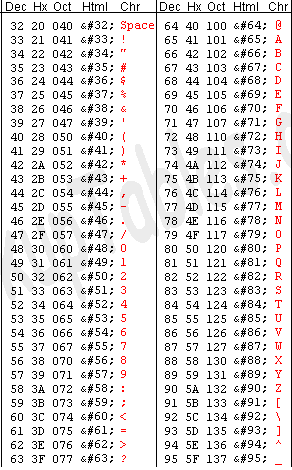
\includegraphics[height=0.7\textheight]{ASCIITABLE.png}
	\caption{Our Elements. \linebreak Taken from: \url{http://www.asciitable.com/}}
	\label{fig:ASCII}
	\end{figure}
\end{frame}

\begin{comment}
\begin{frame}
	\frametitle{Representation of our Elements}
	\begin{itemize}
		\item Each element is encoded as a 6-bit binary string.
		\item We can represent that string as a polynomial in $\mathbb{F}_{2}[x]$.
	\end{itemize}
	
	For example:
	\begin{itemize}
		 \item \# $\rightarrow$ 000011 $\rightarrow x + 1$ 
	\end{itemize}
\end{frame}
\end{comment}

\begin{frame}
	\frametitle{Addition in $\mathbb{F}_{64}$}
	
	\begin{columns}[T]
	
	\begin{column}{.5\textwidth}
	\begin{block}{}
     $\f{!} + \f{ } = \f{!}$\\~\\
	 $\f{!} + \f{!} = \f{ }$\\~\\
	 $\f{!} + \f{"} = \f{\#}$\\~\\
     $\f{1} + \f{2} = \f{\#}$\\~\\
	\end{block}
	\end{column}	
	
	\begin{column}{.5\textwidth}
	\begin{block}{}
		\begin{figure}
	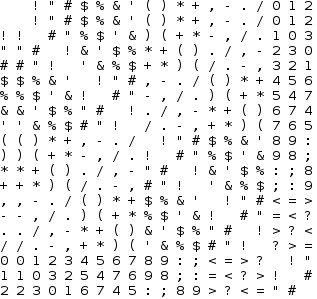
\includegraphics[height=0.5\textheight]{AddTableSection.png}
	\caption{A section of the addition table for $\mathbb{F}_{64}$.}
	\label{fig:Add}
	\end{figure}
	\end{block}
	\end{column}
   
\end{columns}
\end{frame}

\begin{frame}
	\frametitle{Multiplication in $\mathbb{F}_{64}$}

	\begin{columns}[T]
	
	\begin{column}{.5\textwidth}
	\begin{block}{}
		$\f{!} * \f{ } = \f{ }$ \\~\\
		$\f{!} * \f{\#} = \f{\#}$\\~\\
		$\f{\&} * \f{?} = \f{!}$\\~\\
        $\f{3} * \f{A} = \f{H}$\\~\\
	\end{block}
	\end{column}
	
	\begin{column}{.5\textwidth}
	\begin{block}{}
		\begin{figure}
	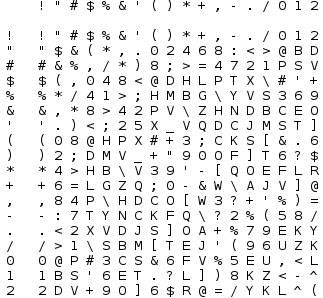
\includegraphics[height=0.5\textheight]{MultTableSection.png}
	\caption{A section of the multiplication table for $\mathbb{F}_{64}$.}
	\label{fig:Mult}
	\end{figure}
	\end{block}
	\end{column}
	
	\end{columns}
\end{frame}

\begin{frame}
	\frametitle{Multiplication in $\mathbb{F}_{64}$}

	\begin{figure}
	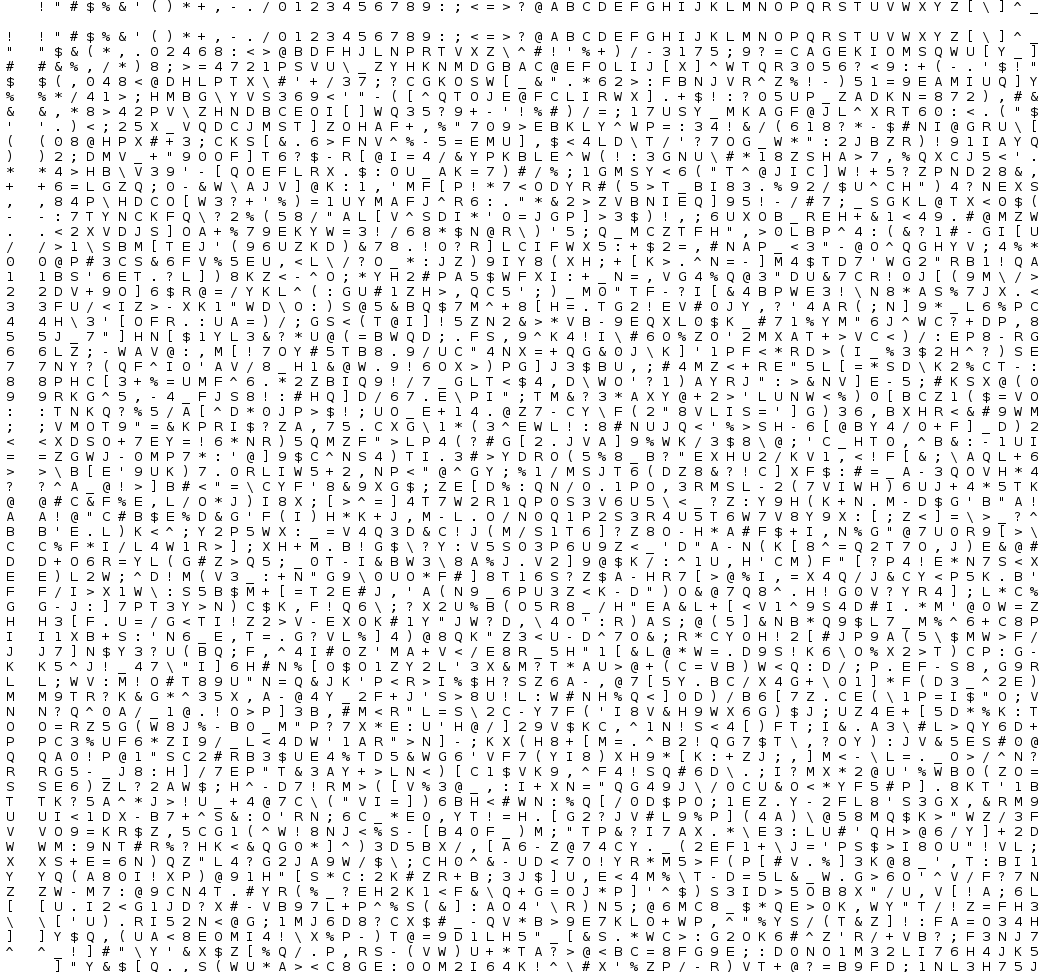
\includegraphics[height=0.7\textheight]{MultTable.png}
	\caption{The complete multiplication table for $\mathbb{F}_{64}$.}
	\label{fig:MultTable}
	\end{figure}

\end{frame}

\begin{frame}
	\frametitle{Multiplication in $\mathbb{F}_{64}$}

	\begin{figure}
	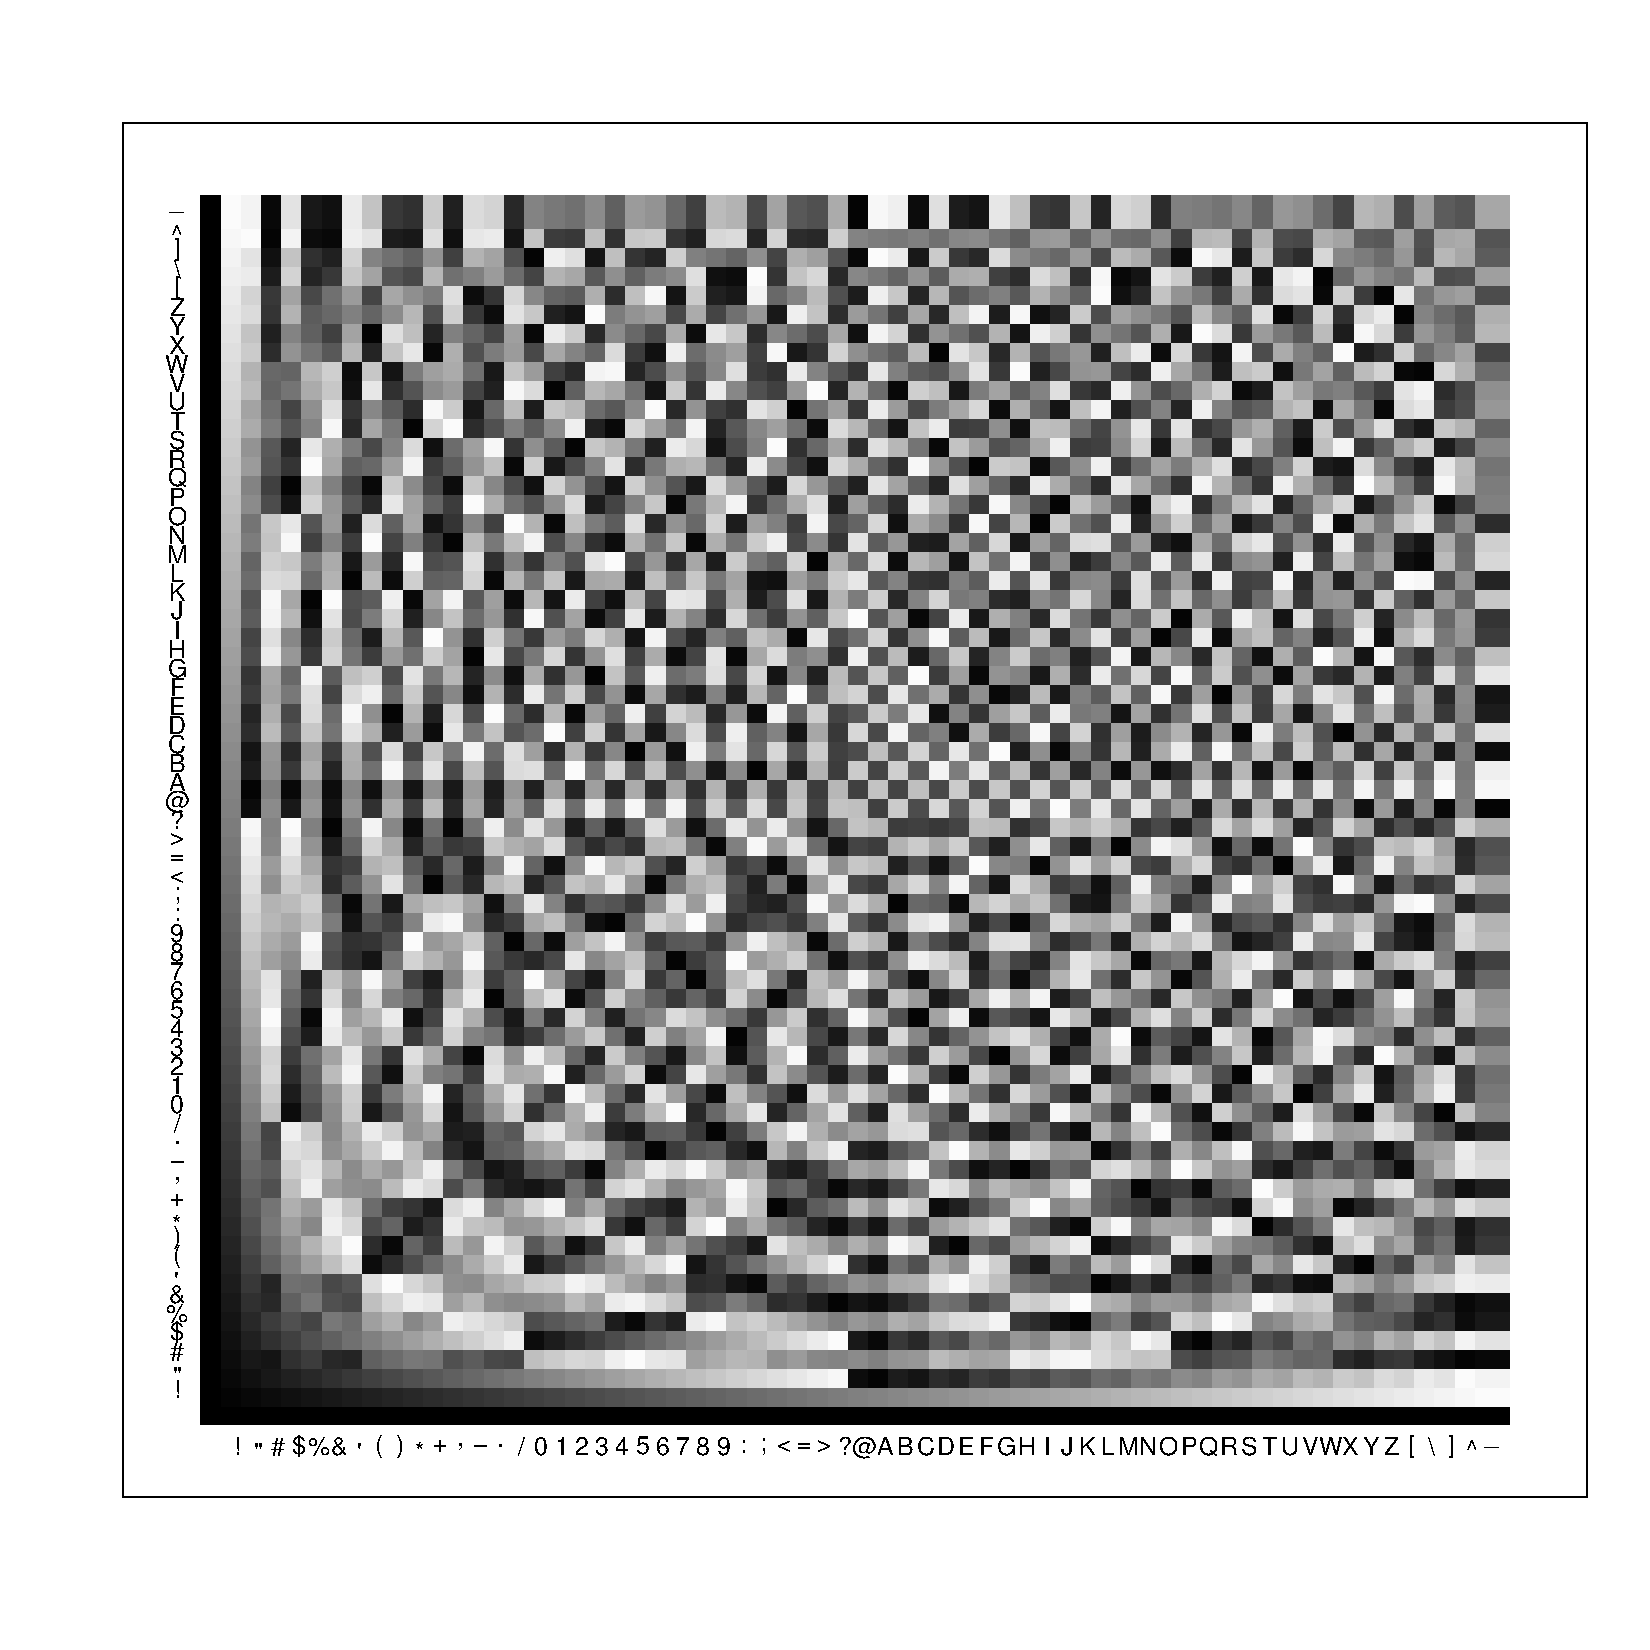
\includegraphics[height=0.7\textheight]{GreyScaleTable.pdf}
	\caption{A greyscale multiplication table for $\mathbb{F}_{64}$.}
	\label{fig:MultTable}
	\end{figure}

\end{frame}

\begin{frame}
	\frametitle{Polynomials over $\mathbb{F}_{64}$}
    Notation:
    \begin{itemize}
    	\item $\mathbb{Q}[x]$ signifies all polynomials with coefficients in $\mathbb{Q}$.
        \item $\mathbb{R}[x]$ signifies all polynomials with coefficients in $\mathbb{R}$.
    \end{itemize}
    Similarly, we write $\mathbb{F}_{64}[x]$ to denote all polynomials with coefficients in $\mathbb{F}_{64}$.\\~\\
    
    $\mathbb{F}_{64}[x]_{k}$ is polynomials of degree less than $k$
    
\end{frame}

\begin{frame}
	\frametitle{Polynomial Multiplication}
	\begin{itemize}
		\item[] $(\f{!}x + \f{\#})(\f{!}x^{2} + \f{"}x + \f{\%})$
        \item[] $= \f{!}x^{3} + \f{"}x^{2} + \f{\#}x^{2} + \f{\%}x + (\f{\#} * \f{"})x + (\f{\#} * \f{\%})$
		\item[] $= \f{!}x^{3} + \f{"}x^{2} + \f{\#}x^{2} + \f{\%}x + \f{\&}x + \f{/}$
        \item[] $= \f{!}x^{3} + \f{!}x^{2} + \f{\#}x + \f{/}$
	\end{itemize}
    Recall: \f{!} is our multiplicative identity.
\end{frame}

\begin{frame}
	\frametitle{Substitution}
	\begin{itemize}
		\item[] $f(x) = \f{!}x^{3} + \f{!}x^{2} + \f{\#}x + \f{/}$
		\item[] $f(\f{A}) = (\f{!} * \f{A}^{3}) + (\f{!} * \f{A}^{2}) + (\f{\#} * \f{A}) + \f{/}$
		\item[] $f(\f{A}) = (\f{!} * \f{Q}) + \f{!} + (\f{\#} * \f{Y}) + \f{/}$
		\item[] $f(\f{A}) = \f{Q} + \f{Y} + \f{@} + \f{/}$
		\item[] $f(\f{A}) = \f{G}$
	\end{itemize}
\end{frame}

\begin{frame}
	\frametitle{Derivative}
	\begin{itemize}
		\item[] $f(x) = \f{!}x^{3} + \f{!}x^{2} + \f{\#}x + \f{/}$
		\item[] $f'(x) = 3 * \f{!}x^{2} + 2 * \f{!}x + \f{\#}$
	\end{itemize}
\end{frame}

\section{Codes}

\begin{frame}
	\frametitle{Introduction to Codes}
	A \textit{code} is a rule for converting information from one representation into another.
	
	\begin{itemize}
		\item $A \rightarrow 1$
		\item $B \rightarrow 2$
		\item $ \vdots $
		\item $Z \rightarrow 26$
	\end{itemize}
\end{frame}

\begin{frame}
	\frametitle{Encoding}
	\textit{Encoding} is the act of conversion, following the rules of the code.
	
	\begin{itemize}
		\item HELLO $\rightarrow$ 8 5 12 12 15
        \item HELLO $\rightarrow$ \f{H}\f{E}\f{L}\f{L}\f{O}
	\end{itemize}
\end{frame}

\begin{frame}
	\frametitle{Errors}
	\textit{Random errors} are a type of error that corrupts individual symbols during transmission.
	\begin{itemize}
		\item \f{\textbf{H}}\f{E}\f{L}\f{L}\f{O} $\rightarrow$ \f{\textbf{J}}\f{E}\f{L}\f{L}\f{O}
	\end{itemize}
	
	\textit{Burst errors} are errors that corrupt a series of contiguous symbols.
	\begin{itemize}
		\item \f{H}\f{\textbf{E}}\f{\textbf{L}}\f{\textbf{L}}\f{O} $\rightarrow$ \f{H}\f{\textbf{\#}}\f{\textbf{F}}\f{\textbf{!}}\f{O}
	\end{itemize}
\end{frame}

\begin{frame}
	\frametitle{Error Correction}
	\textit{Error detecting codes} are a type of code that can detect when these errors occur.
	
	\textit{Error correcting codes} are a type of code that can correct these errors.
\end{frame}

\subsection{Cyclic Redundancy Check}

\begin{frame}
	\frametitle{Introduction to CRC}
	\begin{itemize}
		\item Used to detect accidental changes in data. It cannot correct these errors.
		\item Appends a check value to the message prior to transmission.
		\item After transmission the check value is recomputed and compared to the original value.
	\end{itemize}
\end{frame}

\begin{frame}
	\frametitle{Application and Integrity}
	\begin{itemize}
		\item CRC is good at detecting random errors and burst errors.
		\item It is not suitable for detecting intentional modifications to the data.
	\end{itemize}
\end{frame}

\begin{frame}
	\frametitle{Example}
	To compute a binary CRC with a 3-bit check value:
	\begin{itemize}
		\item Start with our message encoded in binary: 1100101
		\item Make use of a special binary string: 1011
	\end{itemize}
\end{frame}

\begin{frame}[fragile]
	\frametitle{Example}
    \begin{center}
      \begin{verbatim}
          1100101 000
          1011
          0111101 000
           1011
          0010001 000
            1011
          0000111 000
              101 1
          0000010 100
               10 11
         -------------     
          0000000 010
      \end{verbatim}
    \end{center}
\end{frame}

\begin{frame}[fragile]
	\frametitle{Example}
    \begin{center}
      \begin{verbatim}
          1100101 010
          1011
          0111101 010
           1011
          0010001 010
            1011
          0000111 010
              101 1
          0000010 110
               10 11
         -------------     
          0000000 000
      \end{verbatim}
    \end{center}
\end{frame}

\begin{frame}[fragile]
	\frametitle{Example}
    If an error occurs: 
    \begin{center}
      \begin{verbatim}
          1010101 010
          1011
          0001101 010
             1011 
          0000110 010
              101 1
          0000011 110
               10 11
          0000001 000
                1 011
         -------------
          0000000 011
      \end{verbatim}
      Since $011 \neq 010$ we have detected that an error occured.
    \end{center}
\end{frame}

\section{Generalized Reed-Solomon Codes}

\subsection{Reed-Solomon Codes}

\begin{frame}
	\frametitle{History}
	\begin{itemize}
		\item Introduced in 1960 by I.S. Reed and G. Solomon in~\cite{RS:1960}.
		\item Useful in practical applications and mathematically interesting.
		\item Used CD players and deep-space communications.
	\end{itemize}
\end{frame}

\begin{frame}
	\frametitle{The Code}
	Sklar, outlines in~\cite{Sklar:2001} Reed-Solomon Codes
	\begin{itemize}
		\item Reed-Solomon (RS) codes are a type of error correcting code.
		\item A RS-code is capable of correcting $\frac{n - k}{2}$ symbol errors. 
		\begin{itemize}
		 \item $k$ is the number of data symbols
		 \item $n$ is the total number of symbols
		\end{itemize}
		\item Great at correcting burst errors.
	\end{itemize}
\end{frame}

\begin{frame}
	\frametitle{Representation}
	A message encoded using an RS-code is a polynomial with the message symbols embedded in the coefficients. This is called the \textit{message polynomial}.\\~\\
	
	For our example, the message polynomial would be in in $\mathbb{F}_{64}[x]$.
	\begin{itemize}
		\item $\f{H} + \f{E}x + \f{L}x^{2} + \f{L}x^{3} + \f{O}x^{4}$
	\end{itemize}	
	

\end{frame}

\subsection{Generalized Reed-Solomon Codes}

\begin{frame}
	\frametitle{Generalized Reed-Solomon Codes}
	\begin{itemize}
		\item There is an alternate representation, known as Generalized Reed-Solomon (GRS) Codes.
		\item In this representation the message polynomial is evaluated at $n$ distinct points and each is individually scaled. 
		\item The result is a $n$-dimensional vector, which is used as the codeword.
		\item This is the representation that will be used for the remainder of the presentation.
	\end{itemize}
	
\end{frame}

\begin{frame}
	\frametitle{The Code}
	Let $F$ be a field. Choose nonzero elements $\hat{v} = v_{1}, v_{2}...,v_{n} \in F$ and distinct elements $\hat{\alpha} = \alpha_{1}, \alpha_{2}...,\alpha_{n} \in F$.\\~\\
	
	GRS $_{n, k}(\hat{\alpha}, \hat{v}) = \{(v_{1}f(\alpha_{1}),v_{2}f(\alpha_{2}),...,v_{n}f(\alpha_{n}) | f(x) \in F[x]_{k}\}$
	\begin{itemize}
		\item $F = \mathbb{F}_{64}$.
		\item $\hat{v} = (\f{!}, \f{!}, ..., \f{!})$.
		\item $\hat{\alpha} = (\f{A}, \f{B}, ..., \f{W})$.
		\item $f(x)$ is our \textit{message polynomial}.
	\end{itemize}
\end{frame}

\begin{frame}
	\frametitle{Message Polynomial}

	 The message: "THIS IS MAJOR TOM".\\~\\
     
	 $f(x) = \f{T} + \f{H}x + \f{I}x^{2} + \f{S}x^{3} + \f{ }x^{4} + \f{I}x^{5} + \f{S}x^{6} + \f{ }x^{7} + \f{M}x^{8} + \f{A}x^{9} + \f{J}x^{10} + \f{O}x^{11} + \f{R}x^{12} + \f{ }x^{13} + \f{T}x^{14} + \f{O}x^{15} + \f{M}x^{16}$
		

\end{frame}

\subsection{Encoding GRS Codes}

\begin{frame}
	\frametitle{The Codeword}
	The codeword, $\hat{c} = (v_{1}f(\alpha_{1}),v_{2}f(\alpha_{2}),...,v_{n}f(\alpha_{n}))$\\~\\
	$\hat{c} = (\f{!}f(\f{A}),\f{!}f(\f{B}),...,\f{!}f(\f{W}))$\\~\\
	$\hat{c} = (\f{T}, \f{(}, \f{U}, \f{8}, \f{P}, \f{K}, \f{G}, \f{N}, \f{W}, \f{P}, \f{4}, $\\
    \hspace*{4.5ex}   $\f{K}, \f{'}, \f{\_}, \f{N}, \f{(}, \f{M}, \f{H}, \f{K}, \f{1}, \f{"}, \f{<}, \f{K})$
	
\end{frame}

\subsection{Decoding GRS Codes}

\begin{frame}
	\frametitle{The Received Message}
    
    $\hat{c} = (\f{T}, \f{(}, \f{U}, \f{8}, \f{P}, \f{K}, \f{\textcolor{red}{G}}, \f{N}, \f{W}, \f{P}, \f{\textcolor{red}{4}}, $\\
    \hspace*{4.5ex}   $\f{K}, \f{'}, \f{\_}, \f{N}, \f{(}, \f{M}, \f{H}, \f{K}, \f{1}, \f{"}, \f{\textcolor{red}{<}}, \f{K})$\\~\\
	
	$\hat{p} = (\f{T}, \f{(}, \f{U}, \f{8}, \f{P}, \f{K}, \f{\textcolor{red}{Z}}, \f{N}, \f{W}, \f{P}, \f{\textcolor{red}{\&}}, $\\
    \hspace*{4.5ex}   $\f{K}, \f{'}, \f{\_}, \f{N}, \f{(}, \f{M}, \f{H}, \f{K}, \f{1}, \f{"}, \f{\textcolor{red}{R}}, \f{K})$\\~\\
   
    $\hat{c} = \hat{p} + \hat{e}$

\end{frame}

\begin{frame}
	\frametitle{Theorem}
    In~\cite{Hall:2012}, Hall states that there exists $\hat{u} = (u_1, u_2, \ldots, u_n)$ satisfying the following condition:
    
    $\sum\limits_{i=1}^{n} \frac{c_{i}u_{i}}{1 - \alpha_{i}z} = 0 \text{ mod } z^{r}$\\~\\
    
    Where $r = n - k$.
    
\end{frame}

\begin{frame}
	\frametitle{Calculating $\hat{u}$}
	$L(x) = (x - \alpha_{1})(x - \alpha_{2})...(x - \alpha_{n})$\\~\\
	$L_{i}(x) = \frac{L(x)}{(x - \alpha_{i})}$\\~\\
    $\hat{u} = (L_{1}(\alpha_{1}), L_{2}(\alpha_{2}), ... L_{n}(\alpha_{n}),) $\\~\\
	$\hat{u} = (L_{1}(\f{A}), L_{2}(\f{B}), ... L_{23}(\f{W})) $\\~\\
	$\hat{u} = (\f{2}, \f{D}, \f{V}, \f{+}, \f{9}, \f{O}, \f{]}, \f{G}, \f{*}, \f{\^}, \f{3}$
    \hspace*{4.5ex}	    $\f{5}, \f{X}, \f{,}, \f{A}, \f{A}, \f{>}, \f{<}, \f{C}, \f{8}, \f{G}, \f{E}, \f{:}) $\\~\\
\end{frame}

\begin{frame}
	\frametitle{Finding the Syndrome Polynomial}
    We now must calculate the Syndrome Polynomial, $S_{p}(z)$.\\~\\
    
	$S_{p}(z) = \sum\limits^{n}_{i=1} \frac{p_{i}u_{i}}{1-\alpha_{i}z} (\text{mod } z^{r})$\\~\\
    
    $S_{p}(z) = \f{?} + \f{V}z + \f{9}z^{2} + \f{+}z^3 + \f{\^}z^{4} + \f{1}z^{5}$ mod $z^{6}$

\end{frame}

\begin{frame}
	\frametitle{Theorem}
    J. Hall states in~\cite{Hall:2012} that:\\~\\
    Given $r$ and $S_{p}(z) \in F[z]$ there is at most one pair of polynomials $\sigma(z),\omega(z) \in F[z]$ satisfying:
    
    \begin{itemize}
		\item $\sigma(z)S_{p}(z) = \omega(z)$ mod $z^{r}$
        \item deg$(\sigma(z)) \leq r/2$ and deg$(\omega(z)) < r/2$
        \item gcd$(\sigma(z),\omega(z)) = 1$ and $\sigma(0) = 1$
    \end{itemize}

\end{frame}

\begin{frame}
	\frametitle{Introducing $\sigma(z)$ and $\omega(z)$}
    $\sigma(z)$ is called the error locator polynomial\\~\\
    $\omega(z)$ is called the error evaluator polynomial

\end{frame}

\begin{frame}
	\frametitle{The Euclidean Algorithm}
    Due to the previous theorem, and another theorem from~\cite{Hall:2012}, we can use the Euclidean Algorithm to find $\sigma(z)$ and $\omega(z)$.\\~\\
    
    \resizebox{\linewidth}{!}{
    \begin{tabular}{c | c | c | c | c}
		Step i & $q_{i}(z)$ & $r_{i}(z)$ & $s_{i}(z)$ & $t_{i}(z)$ \\ \hline
        -1 & -- & $\f{!}z^{6}$ & $\f{!}$ & $\f{ }$ \\
         0 & -- & $S_{p}(z)$ & $\f{ }$ & $\f{!}$ \\ \hline
         1 & $\f{8} + \f{V}z$ & $\f{\$} + \f{\$}z + \f{\_}z^{2} + \f{6}z^{3} + \f{K}z^{4}$ & $\f{!}$ & $\f{8} + \f{V}z$ \\
         2 & $\f{X} + \f{6}z$ & $\f{Z} + \f{(}z + \f{3}z^{2} + \f{J}z^{3}$ & $\f{X} + \f{6}z$ & $\f{:} + \f{Y}z + \f{\%}z^{2}$ \\
         3 & $\f{C} + \f{Q}z$ & $\f{N} + \f{\_}z + \f{S}z^{2}$ & $\f{N} + \f{I}z + \f{D}z^2$ & $\f{A} + \f{=}z + \f{6}z^{2} + \f{P}z^{3}$\\
        
    \end{tabular}} \\~\\
    
    $\sigma(z) = t_{3}(\f{ })^{-1} t_{3}(z) = \f{!} + \f{Z}x + \f{L}x^2 + \f{C}x^3$\\~\\
    $\omega(z) = t_{3}(\f{ })^{-1} r_{3}(z) = \f{?} + \f{]} + \f{E}x^{2}$\\~\\
    

\end{frame}

\begin{frame}
	\frametitle{Finding the Error Locations}
    The set of error locations, $B$, is defined as: $B = \{b | \sigma(\alpha_{b}^{-1}) = 0\}$\\~\\
    
    $\sigma(z) = \f{!} + \f{Z}x + \f{L}x^{2} + \f{C}x^{3}$\\~\\
    
    The roots of $\sigma$ are: $\f{3}, \f{\%}, \f{1}$\\~\\
    The inverses of the roots are: $\f{G}, \f{K}, \f{V}$ which correspond to the positions 7, 11, and 22 in $\hat{\alpha}$ \\~\\
    $B = \{7, 11, 22\}$
    

\end{frame}

\begin{frame}
	\frametitle{Finding the Error Values}
    The error value $e_{b}$ where $b \in B$ was defined in~\cite{Hall:2012} as:\\~\\
    
    $e_{b} = \frac{-\alpha_{b} \omega(\alpha_{b}^{-1})}{u_{b} \sigma'(\alpha_{b}^{-1})}$\\~\\
    
    $e_{7} = \frac{\f{G} \omega(\f{3})}{\f{]} \sigma'(\f{3})} = \f{=}$\\~\\
    
    $e_{11} = \frac{\f{K} \omega(\f{\%})}{\f{3} \sigma'(\f{\%})} = \f{2}$\\~\\
    
    $e_{22} = \frac{\f{V} \omega(\f{1})}{\f{E} \sigma'(\f{1})} = \f{N}$\\~\\
    
    $\hat{e} = (\f{ }, \f{ }, \f{ }, \f{ }, \f{ }, \f{ }, \f{=}, \f{ }, \f{ }, \f{ }, \f{2}$
    \hspace*{4.5ex} $\f{ }, \f{ }, \f{ }, \f{ }, \f{ }, \f{ }, \f{ }, \f{ }, \f{ }, \f{ }, \f{N}, \f{ })$
    

\end{frame}

\begin{frame}
	\frametitle{Correcting the Errors}
    	
	$\hat{p} = (\f{T}, \f{(}, \f{U}, \f{8}, \f{P}, \f{K}, \f{\textcolor{red}{Z}}, \f{N}, \f{W}, \f{P}, \f{\textcolor{red}{\&}}, $\\
    \hspace*{4.5ex}   $\f{K}, \f{'}, \f{\_}, \f{N}, \f{(}, \f{M}, \f{H}, \f{K}, \f{1}, \f{"}, \f{\textcolor{red}{R}}, \f{K})$\\~\\
    
    $\hat{e} = (\f{ }, \f{ }, \f{ }, \f{ }, \f{ }, \f{ }, \f{=}, \f{ }, \f{ }, \f{ }, \f{2}$
    \hspace*{4.5ex} $\f{ }, \f{ }, \f{ }, \f{ }, \f{ }, \f{ }, \f{ }, \f{ }, \f{ }, \f{ }, \f{N}, \f{ })$\\~\\
    
    $\hat{c} = (\f{T}, \f{(}, \f{U}, \f{8}, \f{P}, \f{K}, \f{\textcolor{red}{G}}, \f{N}, \f{W}, \f{P}, \f{\textcolor{red}{4}}, $\\
    \hspace*{4.5ex}   $\f{K}, \f{'}, \f{\_}, \f{N}, \f{(}, \f{M}, \f{H}, \f{K}, \f{1}, \f{"}, \f{\textcolor{red}{<}}, \f{K})$\\~\\

\end{frame}


\section{Conclusion}

\begin{frame} 
        \frametitle{References} 
        \bibliographystyle{plain}
        \bibliography{bibliography}

\end{frame}

\begin{frame}
	\frametitle{Questions}
\end{frame}

\end{document}